% This is "sig-alternate.tex" V2.0 May 2012
% This file should be compiled with V2.5 of "sig-alternate.cls" May 2012
%
% This example file demonstrates the use of the 'sig-alternate.cls'
% V2.5 LaTeX2e document class file. It is for those submitting
% articles to ACM Conference Proceedings WHO DO NOT WISH TO
% STRICTLY ADHERE TO THE SIGS (PUBS-BOARD-ENDORSED) STYLE.
% The 'sig-alternate.cls' file will produce a similar-looking,
% albeit, 'tighter' paper resulting in, invariably, fewer pages.
%
% ----------------------------------------------------------------------------------------------------------------
% This .tex file (and associated .cls V2.5) produces:
%       1) The Permission Statement
%       2) The Conference (location) Info information
%       3) The Copyright Line with ACM data
%       4) NO page numbers
%
% as against the acm_proc_article-sp.cls file which
% DOES NOT produce 1) thru' 3) above.
%
% Using 'sig-alternate.cls' you have control, however, from within
% the source .tex file, over both the CopyrightYear
% (defaulted to 200X) and the ACM Copyright Data
% (defaulted to X-XXXXX-XX-X/XX/XX).
% e.g.
% \CopyrightYear{2007} will cause 2007 to appear in the copyright line.
% \crdata{0-12345-67-8/90/12} will cause 0-12345-67-8/90/12 to appear in the copyright line.
%
% ---------------------------------------------------------------------------------------------------------------
% This .tex source is an example which *does* use
% the .bib file (from which the .bbl file % is produced).
% REMEMBER HOWEVER: After having produced the .bbl file,
% and prior to final submission, you *NEED* to 'insert'
% your .bbl file into your source .tex file so as to provide
% ONE 'self-contained' source file.
%
% ================= IF YOU HAVE QUESTIONS =======================
% Questions regarding the SIGS styles, SIGS policies and
% procedures, Conferences etc. should be sent to
% Adrienne Griscti (griscti@acm.org)
%
% Technical questions _only_ to
% Gerald Murray (murray@hq.acm.org)
% ===============================================================
%
% For tracking purposes - this is V2.0 - May 2012

\documentclass{sig-alternate}

\usepackage{booktabs,caption,fixltx2e}
\usepackage[flushleft]{threeparttable}
\usepackage{algorithm}
\usepackage{algpseudocode}
\usepackage{pifont}
\usepackage{setspace}
\usepackage{adjustbox}
\usepackage{graphicx}
\usepackage{enumitem}
\usepackage{svg}
\usepackage{amsmath}
\usepackage{multirow}
\usepackage{subfig}
\usepackage{footnote}

\makesavenoteenv{tabular}
\makesavenoteenv{table}

\begin{document}
%
% --- Author Metadata here ---
\conferenceinfo{WOODSTOCK}{'97 El Paso, Texas USA}
%\CopyrightYear{2007} % Allows default copyright year (20XX) to be over-ridden - IF NEED BE.
%\crdata{0-12345-67-8/90/01}  % Allows default copyright data (0-89791-88-6/97/05) to be over-ridden - IF NEED BE.
% --- End of Author Metadata ---

\title{How does personal information reside in human-chosen passwords? \\ --A quantitative study}

% You need the command \numberofauthors to handle the 'placement
% and alignment' of the authors beneath the title.
%
% For aesthetic reasons, we recommend 'three authors at a time'
% i.e. three 'name/affiliation blocks' be placed beneath the title.
%
% NOTE: You are NOT restricted in how many 'rows' of
% "name/affiliations" may appear. We just ask that you restrict
% the number of 'columns' to three.
%
% Because of the available 'opening page real-estate'
% we ask you to refrain from putting more than six authors
% (two rows with three columns) beneath the article title.
% More than six makes the first-page appear very cluttered indeed.
%
% Use the \alignauthor commands to handle the names
% and affiliations for an 'aesthetic maximum' of six authors.
% Add names, affiliations, addresses for
% the seventh etc. author(s) as the argument for the
% \additionalauthors command.
% These 'additional authors' will be output/set for you
% without further effort on your part as the last section in
% the body of your article BEFORE References or any Appendices.

\numberofauthors{3} %  in this sample file, there are a *total*
% of EIGHT authors. SIX appear on the 'first-page' (for formatting
% reasons) and the remaining two appear in the \additionalauthors section.
%
\author{
% You can go ahead and credit any number of authors here,
% e.g. one 'row of three' or two rows (consisting of one row of three
% and a second row of one, two or three).
%
% The command \alignauthor (no curly braces needed) should
% precede each author name, affiliation/snail-mail address and
% e-mail address. Additionally, tag each line of
% affiliation/address with \affaddr, and tag the
% e-mail address with \email.
%
% 1st. author
  % use '\and' if you need 'another row' of author names
% 4th. author
\alignauthor Yue Li\\
       \affaddr{College of William \& Mary}\\
       \email{yli@cs.wm.edu}
% 5th. author
\alignauthor Haining Wang\\
       \affaddr{University of Delaware}\\
       \email{hnw@udel.edu}
% 6th. author
\alignauthor Kun Sun\\
       \affaddr{College of William \& Mary}\\
       \email{ksun@cs.wm.com}
}
% There's nothing stopping you putting the seventh, eighth, etc.
% author on the opening page (as the 'third row') but we ask,
% for aesthetic reasons that you place these 'additional authors'
% in the \additional authors block, viz.
\additionalauthors{Additional authors: John Smith (The Th{\o}rv{\"a}ld Group,
email: {\texttt{jsmith@affiliation.org}}) and Julius P.~Kumquat
(The Kumquat Consortium, email: {\texttt{jpkumquat@consortium.net}}).}
\date{30 July 1999}
% Just remember to make sure that the TOTAL number of authors
% is the number that will appear on the first page PLUS the
% number that will appear in the \additionalauthors section.

\maketitle
\begin{abstract}
Personal information in passwords was understudied due to various reasons. To fill this gap, in this paper we dissect user passwords from a leaked dataset to study how and to what extent do user personal information resides in their passwords. We present most popular password structures as expressed by personal information and show high correlation between passwords and personal information. We also found that male and female behave differently regarding to generating passwords with personal information. Then a quantification metric -- Coverage -- that describes the correlation between passwords and personal information is carried out in this work. Seeing the potential of cracking passwords on top of our analysis, We succeeded developing a semantics-richer Probabilistic Context-Free Grammars method called Personal-PCFG. Personal-PCFG cracks passwords much faster than the state-of-art technique and makes online attacks much easier and more feasible. To defend such semantics-aware attacks, we propose to use distortion functions that are chosen by users to mitigate unwanted correlation between personal information and passwords.

\end{abstract}

% A category with the (minimum) three required fields
\category{}{Security and privacy}{}[Human and societal aspects of security and privacy]
%A category including the fourth, optional field follows...
\category{}{General and reference}{}[Metrics]

\terms{Security}

\keywords{passwords, password cracking, data processing, password protection}

\section{Introduction}
Text-based passwords still remain a dominating and irreplaceable authentication method in foreseeable future. Although people have proposed alternative authentication mechanisms, no such mechanism can bring all benefits of passwords without introducing any extra trouble to users \cite{bonneau2012quest}. However, passwords are also long criticized to be one of the weakest link in authentication system. Numerous works have shown that due to memorability requirement, user passwords are usually far from random strings \cite{bonneau2012science}\cite{malone2012investigating}\cite{narayanan2005fast}\cite{veras2012visualizing}\cite{yan2004password}. For example, "secret" is more likely a human-chosen password than "ziorqpe". As a result, most passwords are within only a small portion of the large password space, making password guessing a lot easier. 

To help both users and system administrators better enhance passwords strength. A very common way is to restrict password creation policies by requiring non-alphabets in passwords. The bad news is that these policies do not keep passwords from vulnerable because users tend to simply mangle their passwords to fulfill the restriction \cite{weir2010testing}, making the security improvement very limited. Nowadays most websites also have password strength meters enabled to provide direct feedbacks to users. However, these meters are proved to be ad-hoc and inconsistent \cite{de2014very}. To better assess the strength of passwords, we need to understand how users construct their passwords. If an attacker knows exactly how users construct their passwords, guessing their passwords will become much easier. On the other hand, if a user knows how other users construct their passwords, the user can easily improve his/her password strength by avoid using these password construction methods. 

Toward this end, researchers have done much to unveil the structures of passwords. Traditional dictionary attacks on passwords have shown that users tend to use simple dictionary words to construct their passwords \cite{hellman1980cryptanalytic}\cite{morris1979password}. Languages users speak are also vital since users tend to use their own languages when constructing passwords \cite{bonneau2012science}. Besides, passwords are mostly phonetically memorable \cite{narayanan2005fast} even they are not simply dicionary words. It is also indicated that users use keyboard strings such as "qwerty" and "qweasdzxc", trivial strings such as "password", "123456", and date strings such as "19951225" in their passwords \cite{li2014large}\cite{schweitzer2009visualizing}\cite{veras2012visualizing}. However, most studies are showing superficial password patterns. The actual composition of passwords are still mysterious to people. Fortunately, an enlightening work studied how users generate their passwords by learning the semantic patterns in passwords \cite{veras2014semantic}. We would like to take another perspective -- personal information, to study password semantics. Based on our analysis and quantification of personal information, we conduct subsequent works on password cracking and protection. 

Our contribution is 4-fold. First, we measure the importance of personal information in passwords and present interesting quantified results. We show most popular password structures with personal information notion embedded. We also found that male and female behave differently when putting personal information in their passwords. Second, we quantify the correlation between user password and personal information by developing a metric -- Coverage. Coverage is useful in measuring password strength, which can potentially be used in password meters. Third, we introduce Personal-PCFG, an evolution of PCFG method by M. Weir\cite{weir2009password} by adding personal information symbols in password structures. Personal-PCFG is able to crack password much faster than PCFG. It also makes online attack more feasible by drastically increasing guessing successful rate with a small amount of guesses. Forth, we discuss how to defend such semantics-aware attacks like Personal-PCFG or \cite{veras2014semantic} by applying a simple distortion function on passwords. 

This paper is organized as follows. Section~\ref{personalinfo} studies how personal information resides in user passwords and shows the gender difference in passwords. Section~\ref{correlationquantification} introduces the Correlation descriptive metric -- Coverage. In Section~\ref{personalpcfg} we present Personal-PCFG and show cracking results compared to original PCFG method. In Section~\ref{passwordprotection} we discussed defense of our attacks by applying distortion functions in passwords.

\section{Personal Info in Passwords}
\label{personalinfo}
Intuitively, people tend to choose their passwords based on their personal information because human beings are limited by their memory -- totally unrelated passwords are much less memorable. We would like to show that user personal experience plays an important role when generating passwords by dissecting passwords in a mid-sized dataset. To start with, we introduce the dataset we use in our study. 

\subsection{12306 Dataset}
In recent years, many password datasets are exposed to the public. Recent works on password measurement or password cracking are usually based on these datasets \cite{bonneau2012science}\cite{li2014large}. Some of these datasets, such as Rockyou, are very large so that they even contain millions of passwords. Now we are going to use a dataset which we call 12306 dataset to illustrate how personal information is used in user passwords.

\subsubsection{Introduction to dataset}
At the end of year 2014, a Chinese dataset is exposed to the public by anonymous attackers. It is reported that the dataset is obtained by attacking using other leaked datasets \cite{tencentnews}, in which attackers use datasets at hand to try other websites. We call this dataset 12306 dataset because all passwords are from a website www.12306.cn. The website is the official website of online railway ticket booking system for Chinese users. There is no data showing the exact number of users in 12306 website. We infer there are at least tens of millions registered users since it is the only official website for the entire Chinese railway systems.

12306 dataset contains over 130,000 Chinese passwords. Having witnessed so many large datasets been leaked out, the size of 12306 dataset is just medium. What makes it special is that together with plain text passwords, the dataset also carries several types of user personal information. For example, user's name, ID number, etc. As the website needs real ID number to register and people need to provide real information to book a ticket, information in the dataset is considered reliable.

\subsubsection{Basic Measurement}
We first do fundamental measurement to reveal some characteristics of 12306 dataset. After appropriate cleansing, we remove a minor part of passwords (0.2\%), with 131,389 good passowrds left for analysis. Note that websites may have different password creation policy. With strict password policy, users may apply mangling rules (For example, $abc -> @bc$ or $abc1$)to their passwords to fulfill the policy requirement \cite{weir2010testing}. As 12306 website has changed its password policy after the password leakage, we do not know exactly the password policy at the time the dataset is leaked. However, from the dataset, we infer the password policy is quite simple -- all passwords need to be no shorter than 6 symbols. There is no restriction on what type of symbols are used. Therefore users are not forced to apply much mangling to their passwords. 

The average length of passwords in 12306 dataset is 8.44. Then we show the most common passwords in 12306 dataset. They are listed in Table~\ref{t1}.
\begin{table}
\centering
\caption{Most Frequent Passwords}
\begin{tabular}{|c|c|c|c|} \hline
Rank&Password&Amount&Percentage\\ \hline
1&123456&389&0.296\%\\ 
2&a123456&280&0.213\%\\ 
3&123456a&165&0.125\%\\ 
4&5201314&160&0.121\%\\ 
5&111111&156&0.118\%\\ 
6&woaini1314&134&0.101\%\\ 
7&qq123456&98&0.074\%\\ 
8&123123&97&0.073\%\\ 
9&000000&96&0.073\%\\ 
10&1qaz2wsx&92&0.070\%\\ 
\hline\end{tabular}
\label{t1}
\end{table}

From Table~\ref{t1} we can see that the dominating passwords are trivial passwords (123456, a123456, etc), keyboard passwords (1qaz2wsx and 1q2w3e4r), and "I love you" type passwords. Both "5201314" and "woaini1314" means "I love you forever" in Chinese. The most commonly used Chinese passwords are similar to previous studies \cite{li2014large}. However, 12306 dataset is much less congregated. The most popular password "123456" counts less than 0.3\% of all passwords while the number is 2.17\% in \cite{li2014large}. We believe that the passowrd sparsity is due to the importance of the website so that users are less prone to use trivial passwords like "123456" and there is few symbil accounts because real ID number is needed. 

Then we show the basic structure of passwords. The most popular password structures are shown in Table~\ref{t2}. Like previous studied \cite{li2014large}, our result again shows that Chinese users prefer to use digits in their passwords instead of letters as in English-speaking users. The 5 top structures all have significant portion of digits, in which at most 2 or 3 letters are appended in front. We reckon that the reason behind may be Chinese users lack vocabulary because Chinese use non-ASCII character set. Digits seem to be the best alternative when creating a password.

\begin{table}
\label{t2}
\centering
\caption{Most Frequent Password Structures}
\begin{tabular}{|c|c|c|c|} \hline
Rank&Structure&Amount&Percentage\\ \hline
1&$D_7$&10893&8.290\%\\ 
2&$D_8$&9442&7.186\%\\ 
3&$D_6$&9084&6.913\%\\ 
4&$L_2D_7$&5065&3.854\%\\ 
5&$L_3D_6$&4820&3.668\%\\ 
6&$L_1D_7$&4770&3.630\%\\ 
7&$L_2D_6$&4261&3.243\%\\ 
8&$L_3D_7$&3883&2.955\%\\ 
9&$D_9$&3590&2.732\%\\ 
10&$L_2D_8$&3362&2.558\%\\ 
\hline\end{tabular}
\begin{tablenotes}
      \small
      \item "D" represents digits and "L" represents English letters. The number indicates the segment length. For example, $L_2D_7$ means the password contains 2 letters following by 7 digits.
    \end{tablenotes}
\end{table}

In conclusion, 12306 dataset is a Chinese password dataset that has general Chinese password characteristics. However, its passwords are more sparse than previously studied datasets. 

\subsection{Personal Information}
As we have mentioned, 12306 dataset not only contains user passwords, it also carries multiple types of personal information. They are:

\begin{verbatim}
1. Name: User's Chinese name
2. Email address: User's registered email address
3. Cellphone number: User's registered cellphone number
4. Account name: the account used to log in the system, 
may contain digits and letters. For example, "myacct123".
5. ID number: Government issued ID number.
\end{verbatim}

Note that the government issued ID number is an 18-digit pretty powerful number. These digits actually show personal information themselves. Digit 1-6 represents the birth place of the owner, Digit 7-14 represents the birthday of the owner, and digit 17 represents the gender of the owner -- odd number means male and even number means female. We take out the 8-digit birthday information and treat it separately because birthday information is very important in a password. Therefore, we finally have 6 types personal information - 1)Name, 2)Birthday, 3)Email, 4)Cellphone 5)Account name, and 6) ID number (birthday is excluded). 

\subsubsection{New Password Representation}
To better illustrate how personal information correlates to user passwords, we develop a new representation of password which add more semantic symbols beside the conventional "D", "L" and "S" symbols, which means digit, letter, and special symbol accordingly. We try to match password to the 6 types of user personal information, and express the passwords with these personal information. For example, a password "alice1987abc" may be represented as $[Name][Birthday]L_3$ instead of $L_3D_4L_3$ as in a traditional measurement. We substitute personal information with corresponding tag ([Name] and [Birthday] in this case). For the segments that are not matched, we still use "D","L", and "S" to describe the types of characters.

We believe representation like $[Name][Birthday]L_3$ is better than $L_5D_4L_3$ since it more accurately describe the composition of user passwords. We would apply the matching process to the whole 12306 dataset to see how these personal information tags appear.

\subsubsection{Matching Method}
\label{matchingmethod}
In order to make personal information password representations, an essential question will be: How do we match the personal information to user passwords? To answer this question, we show the algorithm we used in Algorithm~\ref{alg1}. The high level idea is that we find all substrings of the password and sort them in descending length order. Then we try to match the substrings from longest to shortest to all types of personal information. If one match is found, the leftover password segments are recursively applied the match function until no further match is found. Segments that are not matched to personal information will be then processed using the traditional "LDS" method.


\begin{algorithm}[h!]
\caption{Match personal information with password}
\label{alg1}
\begin{algorithmic}[1]
\Procedure{Match}{$pwd$,$infolist$}
\State $newform \gets$ empty\_string
\If len($pwd$) == 0
\State \Return empty\_string
\EndIf
\State $substring \gets$ get\_all\_substring($pwd$)
\State reverse\_length\_sort($substring$)
\For {$eachstring$ \Pisymbol{psy}{206} $substring$}
\If {len($eachstring$) $\ge$ 2}
\If{matchbd($eachstring$,$infolist$)}
\State $tag \gets $ "[BD]"
\State $leftover \gets pwd$.split($eachstring$)
\State break
\EndIf
\State $\ldots$
\If{matchID($eachstring$,$infolist$)}
\State $tag \gets$ "[ID]"
\State $leftover \gets pwd$.split($eachstring$)
\State break
\EndIf
\Else
\State break
\EndIf
\EndFor
\If{$leftover$.size() $\ge$ 2}
\For{i $\gets$ 0 to $leftover$.size()-2}
\State $newform \gets$ MATCH($leftover[i]$,$infolist$) + $tag$
\EndFor
\State $newform \gets$  MATCH($leftover[leftover.size()-1]$)+$newform$
\Else
\State $newform \gets$ seg($pwd$)
\EndIf
\State \Return $newform$
\EndProcedure
\end{algorithmic}
\end{algorithm}

Note in Algorithm~\ref{alg1} we did not show specific matching algorithm to each type of the personal information (line 10 and line 16) to keep it clean and simple. We describe the matching methods as follows.

First we make sure the password segments are at least of length 2 for matching. For segment of length 1, we directly map it to digit, letter, or special character. We try to match segments with length 2 or more to each kind of the information. For name information, we first convert Chinese names into Pinyin form, which is alphabetic representation of Chinese. Then we compare password segments to 10 possible permutations of the names, which include $lastname + firstname$, $last\_initial+firstname$, etc. If the segment is exactly same as any of the permutations, we consider a match is found. We list all the 10 permutations in the Appendices. For birthday information, we list 17 possible permutations and compare password segments to each of the permutation, if the segment is same as any permutations, we consider a match is found. All the birthday permutations are also listed in the Appendices. For account name, cellphone number, and ID number, we further restrain the length of segment to be at least 4 to avoid coincidence. We believe a match of length 4 is very likely to be an actual match. If the segment is a substring of any of the 3 personal information, we regard it a match to the corresponding personal information. Note that for some password segment, it may match to multiple types of personal information. In this case, each type that matched is counted.


\subsubsection{Matching Result}
\label{matchingresult}
After applying Algorithm~\ref{alg1} to 12306 dataset. We found that 70,892 out of 131,389 (54.0\%) of the passwords contain at least one of the 6 types of personal information. Apparently, personal information is an essential part of user passwords and most users put certain personal information in their passwords. We believe the rate could be higher if we have more personal information at hand. However, this percentage has served its purpose properly. We present the top 10 password structures in Table~\ref{t3} and most commonly used personal information in Table~\ref{t4}. As we have mentioned before, some password segment may match to multiple types of personal information and we count each matched type. Therefore with 131,389 passwords we obtain 143373 password structures. Based on Table~\ref{t3} and Table~\ref{t4}, we have the following observations

\begin{table}
\centering
\caption{Most Frequent Password Structures}
\begin{tabular}{|c|c|c|c|} \hline
Rank&Structure&Amount&Percentage\\ \hline
1&D7&7122&5.420\% \\
2&[ACCT]&6820&5.190\% \\
3&[NAME][BD]&5410&4.117\% \\
4&D6&4886&3.718\% \\
5&[BD]&4470&3.402\% \\
6&D8&4245&3.230\% \\
7&[EMAIL]&3807&2.897\% \\
8&L1D7&3296&2.508\% \\
9&[NAME]D7&2949&2.244\% \\
10&[NAME]D3&2363&1.798\% \\
\hline\end{tabular}
\label{t3}
\end{table}

\begin{table}
\centering
\caption{Most Popular Personal Information}
\begin{tabular}{|c|c|c|c|} \hline
Rank&Information Type&Amount&Percentage\\ \hline
1&[BD]&32373&24.63\%\\
2&[NAME]&29646&22.56\%\\
3&[ACCT]&21324&16.22\%\\
4&[EMAIL]&11020&8.387\%\\
5&[ID]&1210&0.920\%\\
6&[CELL]&634&0.482\%\\
\hline\end{tabular}
\label{t4}
\end{table}

\begin{enumerate}[leftmargin=*]
\item The second and third structures are perfectly matched to personal information. 3 out of the top 10 structures are composed by pure personal information and 6 out of the top 10 structures have personal information segment. The dominating structures $D_7$, $D_6$, and $D_8$ in Table~\ref{t2} still rank fairly high.
\item Birthday, name, and account name are most popular personal information in user passwords. Over 20\% passwords in our dataset contain birthday or name information. On the other hand, much less people use email and ID number in their passwords. Further more, only few people include their cellphone number in their passwords.  
\item Set aside personal information, digits are still dominating user passwords. Only one structure from the top 10 structures has one letter segment with minimum length (1). The result confirms that Chinese users prefer to use digits in their passwords.
\item An interesting observation is that although account name has merely half percentage as birthday and name information, the structure [ACCT] ranks highest among all structures that contain personal information. The reason behind may be that users tend to use their account names as their entire passwords instead of using them as part of their passwords. 
\item Users seem not like applying mangling rules on their passwords. We notice that the several most frequent password structures are either pure personal information (such as $[BD]$) or pure strings (such as $D_6$) that do not relate to any of the personal information. Structures like $[NAME]D_7$ are less likely to appear in user password.
\end{enumerate}

\subsubsection{Gender difference}
\label{genderdifference}
Beside treating the dataset as a whole entity, it is also interesting to study the difference of password structures between males and females. Although the dataset does not have a gender column, user ID number actually has gender information (The second last digit in ID number represents gender). However, we found that the dataset is biased in gender, with 9,856 females and 121,533 males in it. To balance the number, we randomly select 9,856 males from the male pool and compare them with females. 

The average length of passwords for males and females are 8.41 and 8.51, which are quite similar. It shows that males and females do not differ much in the length of their passwords. We then apply the matching method to each of the genders. We found that 54.9\% of male passwords contain personal information while only 44.6\% of female passwords contain personal information. Besides, the number of structures of female passwords is 1,194, which is 8.7\% more than the number of male passwords. Therefore we conclude that generally males put more personal information in their passwords than females do. It also implies that females have more complex passwords, and therefore maybe more secure. We list the top 10 structures for each gender in Table~\ref{t5} and personal information usage in Table~\ref{t6}. From the tables we have the following observations:
\begin{enumerate}[leftmargin=*]
\item The top 10 structures count 33.62\% of males passwords and 28.31\% of female passwords. Besides, the total number of password structures of males is also smaller. We can see passwords of males are more congregated, and therefore more predictable. 
\item For males, 6 out of the top 10 structures contain personal information. Yet for females, only 3 out of top 10 structures contain personal information. It further implies that males are more likely to consider personal information when creating passwords.
\item For both males and females, [ACCT], [NAME][BD], and [BD] are three most frequent structures with personal information. However, The percentage of males are much higher than that of females. Averagely 47.3\% more males are constructing their passwords following the 3 patterns than females.
\item From Table~\ref{t6} we can see the percentage of each type of personal information in the passwords. Interestingly males and females are very different in the usage of name information. Males use their names as frequent as their birthday (23.43\% passwords of males contain their names) while only 13.03\% passwords of females contain names. We also notice that the name usage mostly contribute the 10\% difference in personal information usage between males and females. 
\end{enumerate} 

\begin{table}
\centering
\caption{Most Frequent Structures in Different Gender}
\begin{adjustbox}{max width=0.48\textwidth}
\begin{tabular}{|c|c|c|c|c|} \hline
\multirow{2}{*}{Rank}&\multicolumn{2}{|c|}{Male}&\multicolumn{2}{|c|}{Female}\\ \cline{2-5}
&Structure&Percentage&Structure&Percentage\\ \hline
1&$D_7$&5.752\%&$D_6$&4.890\%\\
2&[ACCT]&5.418\%&$D_7$&4.220\%\\
3&[NAME][BD]&4.190\%&[ACCT]&4.210\%\\
4&[BD]&3.591\%&$D_8$&3.256\%\\
5&$D_6$&3.530\%&[EMAIL]&2.678\%\\
6&[EMAIL]&2.962\%&[NAME][BD]&2.607\%\\
7&$D_8$&2.861\%&[BD]&2.221\%\\
8&$L_1D_7$&2.851\%&$L_2D_6$&2.079\%\\
9&[NAME]$D_7$&2.353\%&$L_2D_7$&1.704\%\\
10&[NAME]$D_6$&1.978\%&$L_1D_7$&1.684\%\\
\hline\end{tabular}
\end{adjustbox}
\label{t5}
\end{table}

\begin{table}
\centering
\caption{Most Frequent Personal Information in Different Gender}
\begin{adjustbox}{max width=0.48\textwidth}
\begin{tabular}{|c|c|c|c|c|} \hline
\multirow{2}{*}{Rank}&\multicolumn{2}{|c|}{Male}&\multicolumn{2}{|c|}{Female}\\ \cline{2-5}
&Information Type&Percentage&Information Type&Percentage\\ \hline
1&[BD]&25.02\%&[BD]&21.14\%  \\
2&[NAME]&23.43\%&[ACCT]&15.35\%\\
3&[ACCT]&16.27\%&[NAME]&13.02\%\\
4&[EMAIL]&7.96\%&[EMAIL]&8.81\%\\
5&[ID]&1.02\%&[ID]&0.45\%\\
6&[CELL]&0.30\%&[CELL]&0.41\%\\
\hline\end{tabular}
\end{adjustbox}
\label{t6}
\end{table}

In conclusion, passwords of males are generally composed of more personal information, especially names of the users. The sparsity of passwords of males is lower. We believe insightful analysis on the difference between male and female passwords is interesting since it provides insight for both password cracking and protection. 


\subsection{Service Information} 
Cao et al \cite{cao2014personalized} propose an interesting idea that use service information to crack user passwords. However, the idea has not been carried out with an experiment. It draws our interest because we have shown the importance of personal information in user password and naturally we are also interested in how important the service information can be in user passwords. By service information we mean the information of service provider. For example, the famous "Rockyou" dataset is leaked from a website $www.rockyou.com$, the service information could be "rockyou". In our case, the service information is "12306". It is reasonable for a user to add service information to their passwords to keep his/her passwords different in each site. The approach balances password security and memorability. Therefore we wish to verify whether service information is as important as personal information. As 12306 is just a medium-sized Chinese dataset, the result may not be very representative. Therefore, we would like to verify more datasets, including Tianya dataset and Rockyou dataset, etc. in each of the datasets, we try to search the service information in the passwords. The result is shown in Table~\ref{t7}.

\begin{table}[!]
\centering
\caption{Service Information in Passwords}
\begin{adjustbox}{max width=0.48\textwidth}
\begin{tabular}{|c|c|c|c|} \hline
Dataset & Password Amount & Service info Amount & Percentage\\ \hline
Rockyou & 14,344,391 & 44,025 & 0.3\%\\ 
Tianya & 26,832,592 & 29,430{ \footnote{We found 45,574 passwords in Tianya dataset is "111222tiany". It does not make much sense for so many user using such same password so we doubt they are mostly sybil accounts. Therefore the duplications are removed in our analysis} } &0.11\%\\ 
PHPBB & 184,389 & 2,209 & 1.2\%\\ 
12306 & 131,389 & 490 & 0.4\%\\ 
MySpace & 37144 & 72 & 0.2\%\\ 
\hline\end{tabular}
\end{adjustbox}
\label{t7}
\end{table}

As shown in Table~\ref{t7}, we can see indeed some users are using service information in their passwords. Our results indicate that all datasets examined contain 0.11\% to 1.2\% passwords that relate to service information. However, the portion is quite small. Such small percentage indicates that though adding service information in user passwords may maintain good memorability and security, currently few users are using such method to construct their passwords. Therefore, we concluded that only few users include service information in their passwords. the method proposed by Cao et al that uses service information to crack passwords may not bring much improvement over state-of-art technique.


\subsection{Ethical Consideration}
We do realize that studying leaked datasets involves much ethical concern. We claim that we only use the datasets for researching purpose. All data are carefully stored and used. We will not expose any user personal information or password or use these information in any other way except for research use.

\section{Correlation Quantification}
\label{correlationquantification}
In Section~\ref{matchingresult} we have shown the personal-information-involved password structure distributions and how much does each type of the personal information count in all passwords. These results helped us to draw interesting qualitative conclusions such as users like to use their personal information in their passwords and quantitative conclusions such as birthday appears in 24.63\% passwords, which is the highest percentage among the 6 types of personal information.
However, until this point we do not have a clear idea about how much does personal information correlate to passwords in a quantitative way. Although we have shown useful numbers between each type of personal information and passwords (such as birthday appears in 24.63\% passwords), these numbers are not ideal to describe the passwords because there are many of them. Yet we seek a more comprehensive method to quantify the correlation between passwords and personal information. Thereby we create a new metric -- Coverage -- to quantify the correlation. 

\subsection{Coverage}
\label{coverage}

Coverage is a useful metric to describe how close are personal information and passwords. It is used on every individual user in the dataset. The average Coverage also reflects correlation of the dataset. We will show the computation of coverage and give a detailed example in the following section to illustrate how Coverage works. Besides, we also explain why Coverage is a good metric to describe the correlation between password and all personal information available. 
\subsubsection{Computation Method}
\label{computationmethod}
To compute coverage, we take password and personal information in terms of strings as input. And we use a sliding window approach as in data transmission protocols to compute Coverage. We maintain a dynamic-sized window sliding from the beginning to the end of the password. The initial size of the window is 2. If the segment in the window matched to a certain type of personal information, we enlarge the window by size of 1. Then we try again to match the segment in the window to personal information. If a match is found, we further enlarge the window size until matches no longer exist. At this point we slide the window by one symbol and reset the window size to be the initial size. In the mean time of sliding, we maintain an array of same length as the password. This array is called tag array. Tag array is used to record the length of each matched password segment. For example, a tag array may be [4,4,4,4,0,0,2,2]. This array implies that the first 4 password symbols match certain type of personal information. the 5th and 6th symbols have no match and the last 2 symbols also match certain type of personal information. It does not matter which type do first 4 symbols and last 2 symbols match. When we eventually slide window through the password string thoroughly, the tag array is used to compute the Coverage metric. Coverage is computed as the sum of squares of matched password segment length divided by the square of password length. Mathematically
\begin{equation} \label{eq1}
\begin{split}
CVG & = \sum_{i=1}^n (\frac{l_n^2}{L^2}) \\
\end{split}
\end{equation}
in which $n$ means the number of matched password segment, $l_n$ means the length of corresponding matched password segment, and $L$ means the length of the password. We show the algorithm that is used to compute Coverage in Algorithm~\ref{alg2}. Note that differently from the matching algorithm introduced in Section~\ref{matchingmethod}, we aim to keep the matching for Coverage simpler in order to keep it universally applicable. Namely we try to keep ad-hoc processing on each type of personal information minimum. Toward this end, we do not include various composition of birthday. Cases like DD+MM+YYYY are ignored and we keep only the only case of YYYY+MM+DD, which conforms to Chinese conventions. However, we keep full name and name initials to match names because name initials are very common in Chinese passwords. Besides, only little processing is acceptable in computation of Coverage. As a conclusion, only names have 2 permutations, other personal information keep their original format. A match is found if a password segment is a substring of any of the personal information.


\begin{algorithm}[!]
\caption{Compute Coverage}
\label{alg2}
\begin{algorithmic}[1]
\Procedure{Cvg}{$pwd$,$infolist$}
\State $windowsize \gets$ 2
\State $pwdlen \gets$ len($pwd$)
\State $matchtag \gets$ [0]*$pwdlen$
\State $matchmark \gets $ 0
\State $cvg \gets $ 0
\While {$windowsize \le $len($pwd$)}
\State $passseg \gets pwd[0:windowsize]$
\If {$passseg$ = substring of $infolist$}
\For {$j \gets matchmark$ to $matchmark$+$windowsize$}
\State $matchtag[j] \gets windowsize$
\EndFor
\If {$windowsize$ != len($pwd$)}
\State $windowsize \gets windowsize$+1
\EndIf
\Else
\State $matchmark \gets matchmark$+$windowsize$
\State $pwd \gets pwd[windowsize:]$
\State $windowsize \gets$ 2
\EndIf
\EndWhile
\For {$eachitem$ in $matchtag$}
\State $cvg \gets cvg + eachitem$
\EndFor
\State \Return $cvg/(pwdlen * pwdlen)$
\EndProcedure
\end{algorithmic}
\end{algorithm}

We illustrate a simple example in Figure~\ref{f1}. In this example, we take a user named Alice, who was born in Aug. 16, 1988. Her password happens to be "alice816". If we apply the algorithm in Section~\ref{matchingresult}, the structure of this password will be [NAME][BD]. Apparently her password is quite related to her personal information. To quantify this relation, we follow Algorithm~\ref{alg2} to compute Coverage for her in each step as shown in Figure~\ref{f1}. (a) The password is prepared for a window to slide through. Note the personal information include "alice" as name and "19880816" as birthday. The tag array is initialized as [0 0 0 0 0 0 0 0]. (b) Window size is initialed to 2 so the first 2 symbols in the password are covered. "al" is a substring of alice's name, so a match is found. Therefore we extend the window size by 1 and the tag array is updated as [2 2 0 0 0 0 0 0]. (c)-(e) Window keeps growing because matches are continuously found. The tag array also keeps updating. (f) The window now covers "alice8", which is not a substring of "alice" or "19880816". Therefore, window size is rest to 2 and tag array remains unchanged. (g) The window of size 2 now covers "81", which is a substring of birthday, again we extend the window by 1 and update tag array to [5 5 5 5 5 2 2 0] (h) After window grows, "816" is also found a match. Tag array is updated to [5 5 5 5 5 3 3 3]. The window does not grow or slide any more because it has reached the end of the password. (i) All symbols have settled. Tag array can now be used to compute Coverage. Based on Equation~\ref{eq1}, the coverage is computed as $CVG  = \sum_{i=1}^2 {{l_n^2} \over {L^2}} = {{5^2 + 3^2}\over{8^2}}= 0.52$.

\begin{figure}[h!]
\centering
  \caption{Coverage - An Example}{}
  \label{f1}
  \centering
    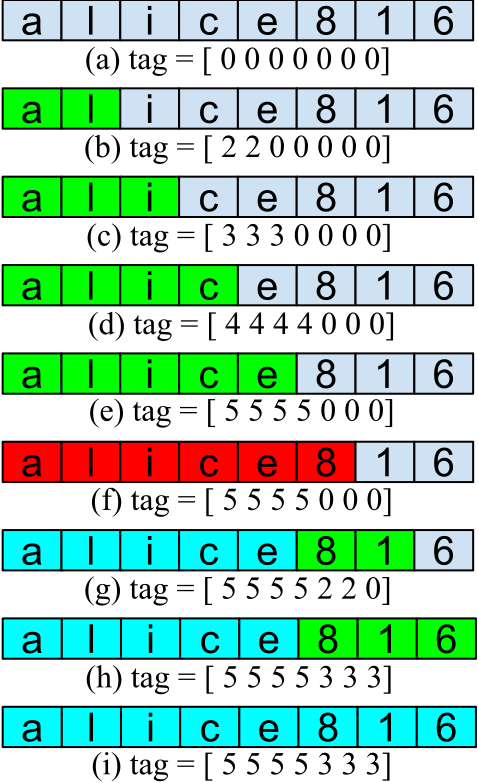
\includegraphics[width=0.3\textwidth]{fig/cvgfig}
\caption*{Grey boxes hold unvisited password symbols. green and red boxes denote that the symbols inside are covered by the sliding window. White boxes denote the symbols inside have been settled (window stops extending). }

\end{figure}


In order to show that Coverage is a useful and reasonable metric, we present 4 features that Coverage has and why we need these features.

\begin{enumerate}[leftmargin=*]
\item By the nature of Equation~\ref{eq1}, Coverage ranges from 0 to 1, in which 0 means no personal information is matched to any password segment and 1 means the entire password is matched to only one type of personal information. 
\item Coverage can be universally applicable for its simplicity. Any kind of personal information can be formatted as a string, check whether or not a password segment is a substring of the string is straightforward. Besides, a few variations of personal information strings may be applied to enhance the completeness and accuracy (like names in our application). Therefore, even certain types of personal information are missing or extra types of personal information are available, Coverage can consistently serve its purpose.
\item Coverage can reflect the length of personal information over the length of password. We need this feature because longer matched password segment naturally indicates stronger correlation. From Equation~\ref{1}, for a matched password segment, the longer the segment is, the larger the numerator will be. It is obvious Coverage measures the correlation strength. \item For personal information segments of same length, Coverage stresses the Continuation of matching. We argue that continuous match is stronger than fragmented match. That is to say, for a given password of length $l$, a matched segment of length $l$ has stronger password than 2 matched segments of length $l_1$ and $l_2$ with $l = l_1 + l_2$. For example, a matched segment of length 6 is expected to have stronger correlation than 2 matched segments of length 2 and 4. We desire this feature because shorter segments usually involve wrong match (coincidence). Since it is very hard to differentiate a real match and a coincidence match, we would like to minimize the effect of wrong matches by taking squares of the matched segments to compute the Coverage.
\end{enumerate}

\subsection{Result}
We apply Algorithm~\ref{alg2} on every user of 12306 dataset. The result is shown as a cumulative distribution graph in Figure~\ref{f2}. From the figure we have the following observation
\begin{enumerate}[leftmargin=*]
\item Half of the users have Coverage higher than 0.186, implying that  a significant portion of user passwords have relatively high correlation to their personal information.
\item 9.9\% users have 0 Coverage. 0 Coverage indicates there is no possible correlation between the users' passwords and their personal information.
\item 10.5\% users have Coverage of 1, which means that 11.9\% passwords are perfectly matched to exactly one type of personal information. However, Only 13.4\% users have Coverage higher than 0.5 and lower than 1.0. 
\end{enumerate}

\begin{figure}[h!]
\centering
  \caption{Coverage distribution}{}
  \label{f2}
  \centering
    \includegraphics[width=0.45\textwidth]{fig/cvghist}
\end{figure}

Besides, the average Coverage for 12306 dataset is 0.309. We also compute the average Coverages for male and female groups that are used in Section~\ref{genderdifference}, in which we concluded that male users are more likely to include personal information in their passwords. It turns out that the average Coverage for male group is 0.314 and the average Coverage for female group is 0.269. Our result indicates that the correlation between password and personal information for male users is higher. It complies with our previous conclusion. Therefore, it shows that Coverage works well to determine the correlation between passwords and personal information.

\subsection{Coverage Usage}
Coverage can be used in many scenarios. Firstly, it can be used as a reserach metric to describe a dataset. Coverage directly reflects the correlation between password and available personal information. Investigating how users from different systems behave regarding to constructing their passwords using personal information would be an interesting future work. 

Apparently, Coverage would be very useful in password strength meters. Strength meters are reported as mostly ad-hoc \cite{de2014very}. Most meters dumbly give score based on password structures and length, or blacklist commonly used passwords (such as "password"). There are also meters that do simple social profile analysis such as passwords cannot have the users' names or passwords cannot be the same as account names. However, these simple analysis mechanisms can be easily fooled by mangling the password a little. In cases of password strength meters, Coverage is able to cover the unnoticed corner of personal information. Consider the routine for creating an account. Users usually fill in some profile information such as name, birthday, email address, etc and create a password. At this moment password meters will offer feedback of password strength normally in bar forms. Since personal information is available, it is straightforward to set Coverage as part of strength measurement. Apparently, higher Coverage indicates vulnerable passwords. Systems can even ban passwords when they surpass a preset Coverage threshold. Additionally, users cannot easily escape Coverage measurement by simple mangling, thus their passwords are further secured. 

Coverage can also be added to existing tools to enhance their capabilities. There are several Markov Model based tools that predict the next character when the user creates a password \cite{komanduri2014telepathwords}\cite{weir2010testing}. Users would be surprised to find that the next character in their mind matches exactly the tool output and then switch to a more unpredictable passwords. Coverage is able to work in these tools as an enhancement -- When Coverage is rather high, it is easy to predict what the next character of user input is.



\section{Personal-PCFG, an individual oriented password cracker}
\label{personalpcfg}
We have presented abundant findings regarding user personal information and their passwords, as well as a metric to quantify their correlation. Naturally we wonder how are these findings useful. And an obvious answer is that given there is significant correlation between user password and personal information, we can make password cracking much faster. Therefore we create Personal-PCFG, which relies on the idea of PCFG approach created by M. Weir \cite{weir2009password}. However, unlike original PCFG method, Personal-PCFG is an individual-oriented password cracker. It generates personalized guesses towards each user.

\subsection{Attack Scenarios}
Personal-PCFG can be used in both offline and online attacks. Attackers need to know certain amount of personal information about the targets. The attackers can be an evil neighbor, a curious friend, a jealous husband, a blackmailer (for online attacks). Or even a company that buys personal information from other companies (for offline attacks). Under these conditions, target personal information is rather easy to obtain -- The attackers might either know some victim personal information or can easily get personal information by searching online, especially social networks sites (SNS). 

In traditional offline password attacks, attackers usually steal hashed passwords from victim systems, and try to find out the unhashed values of these passwords. As hash process cannot be simply reversed, the most usual solution is by brute force, namely guessing and verifying passwords. Every guess is verified by hashing the guess (salt is also likely to be added) and comparing it to each of the hashed values. high-probability password guesses can usually match many hashed values and thus are usually tried first. In offline attacks, Personal-PCFG is much faster in guessing out the correct password than conventional methods by generating high-probability personalized passwords.

As for online attack, the attacker does not even have a hashed database. Instead the attacker tries to directly log in the real systems. It is considered more difficult than offline attacks because websites usually have restrictions on log in attempts for a given period of time. If the trial quota has been reached without inputting the correct password, the target account may be locked either for some time or permanently unless certain actions are taken (For example, call the service provider). As a matter of fact, online attacks need to be very fast -- within at most tens of guesses the password should be cracked out. Any proposed password cracking method 

\subsection{A revisit of PCFG}
Personal-PCFG method is based on the idea of PCFG method. Before we introduce Personal-PCFG. We revisit the basic principle of PCFG method. PCFG method pre-processes passwords by their structures. From the pre-process base structures such as $"L_5D_3S_1"$ are generated for each of the passwords. Then PCFG method substitute the "D" and "S" segments using segments of same length learned from the training set. These substitute segments are ranked by probability of occurring in training set. Therefore higher probability segments will be tried first. For example, "123" is a high-probability candidate for $D_3$ while "691" may not be a high probability candidate. As a result, one base structure may have many substitutions, for example, $"L_5D_3S_1"$ can have $"L_5123!"$ and $"L_5691!"$, etc as its substitutions. These new representations are called pre-terminal structures. No "L" segment is substituted because the space of alpha strings is too large to learn from the training set. These pre-terminals are ranked from high probability to low probability. And finally "L" segments are substituted using a dictionary. Besides the basic idea, PCFG method also carries an efficient algorithm to enumerate passwords from high probability to low probability on the fly, which will also be used in Personal-PCFG. Therefore PCFG method generates password guesses in descending probability order. These guesses are hashed to compare with the values in password databases. Since PCFG method output statistically high probability password first. It reduces the guessing number of traditional dictionary attacks significantly. 

\subsection{Personal-PCFG}
Personal PCFG leverages the basic idea of PCFG method. Beside "L", "D", and "S" symbols, it adds more semantic symbols to PCFG method. These additional symbols include "B" for birthday, "N" for name, "E" for email address, "A" for account name, and "I" for id number. More semantics makes Personal-PCFG more accurate in predicting passwords. To make Personal-PCFG work, additional matching phase and adapt-substitution phase are added to the original PCFG method. Personal-PCFG works as following.
\subsubsection{Matching}
Given a password string, we first try to match it or a substring of it to personal information. The algorithm used is the same as that introduced in Section~\ref{matchingmethod}. However, this time we also record the length of the matching segment. We replace the matched segments in password with corresponding symbols and length. Unmatched segments will remain unchanged. Again, We take Alice, who was born in Aug. 16 1988, as an example. This time we assume her password is "helloalice816!". Matching phase will replace "alice" with "$N_5$" and "816" with "$B_3$. The leftover is kept unchanged. Thereby the outcome of this step is "$helloN_5B_3!$" 
\subsubsection{Processing}
In this step we simply run the processing routine of original PCFG method on the output of last step. The segments that are matched to personal information are not processed in this step. The output in this step is a base structure for Personal-PCFG. Now the password is fully described by symbols of Personal-PCFG method. Our example password "$helloN_5B_3!$" will update to "$L_5N_5B_3S_1$". 
\subsubsection{Guess Generation}
Like original PCFG method, we replace "D" and "S" symbols with actual strings learned from the training set in descending probability order. "L" symbols are also replaced with words from a dictionary. We use the "NEXT" function in [] to output the results on the fly so we do not need to wait all possibilities for guesses are calculated and sorted. The results will be kept outputting for next step. Note that we do not replace any symbols for personal information so the guesses are still not actual guesses. We do not handle personal information in this step because personal information for each user is likely to be different. Personal information symbols can only be substituted when the target is specific. In this step our base structures generate pre-terminals, which are partial guesses that contain part of actual guesses and part of Personal-PCFG symbols. The example "$L_5N_5B_3S_1$" is now "$helloN_5B_3!$". if "hello" is the first 5 symbols long string in the input dictionary and "!" has highest probability of occurring for 1 symbol long special character strings in the training set. Note that for "L" segments, every words of same length has same probability. The probability of "hello" is simply $1\over N$, in which $N$ is the total number of words of length 5 in the input dictionary. 

\subsubsection{Adapt-substitution}
The result of last step can be applied to any target user. However, this will no longer be true in this step because the guesses will be further substituted with personal information, which are specific to only one target user. Personal information symbols are replaced by corresponding personal information of same length. If there are multiple candidates of same length, every combination is output for trial. In our example guess $helloN_5B_3!$, $N_5$ will be directly replaced by "alice". However, $B_3$ has many candidate segments. Any length 3 substring of "19880816" can be a candidate. Therefore every substring will be output. The guesses are "helloalice198!", "helloalice988!", $\ldots$, "helloalice816!". We know the final try is exactly the password of Alice. Note that on the opposite of having multiple candidate, not all personal information segments can be replaced because same length segments may not always be available. For example, a $helloN_6B_3!$ is not suitable for Alice for her name is at most 5 symbols long. In this case no guess from this pre-terminal structures will be output for Alice. 

\subsection{Cracking Result}
We use 12306 dataset in both Personal-PCFG and original PCFG method. 12306 dataset has 131,389 users. We use half of them as training set, and the other half as testing set. Besides, both of the methods involve selection of dictionaries for the "L" segments. Dictionaries are a vital part for password cracking. [] proved that vocabulary in password datasets are more closed to each other than to an ordinary dictionary therefore using dictionaries collected from other dataset is more efficient. To eliminate the effect of unfair dictionary selection, we use "perfect" dictionaries in both of the methods. "Perfect" dictionaries are dictionaries we collected directly from the testing set, in which any string is useful and no string is uncovered. Therefore a perfect dictionary is guaranteed to find correct alpha strings efficiently.

We realized that most previous works on password cracking use guessing number to compare different methods. However, we use hashing number to evaluate Personal-PCFG. We argue that as hashing is the bottleneck of such attacks, it is more reasonable to compare hashing number instead of guessing number. It is acceptable to use guessing number in past works because guessing number has linear relation to hashing number. For each guess, it needs to be padded by the salt before hashing. Therefore, a database of $N$ passwords requires $N$ hashes to verify each guess. However, in Personal-PCFG, one guess is usually personalized to test on only one password so it requires only $1$ hash to verify a guess. Therefore insist on using guessing number to compare 2 methods is inappropriate.

The result is shown in Figure~\ref{f3}, in which we compute the percentage of a password that can be cracked given the guessing number. We found that Personal-PCFG works substantially better than original PCFG method. Some interesting observations are listed in following.

\begin{figure}[h!]
\centering
  \caption{Compare PCFG and Personal-PCFG}{}
  \label{f3}
  \centering
    \includegraphics[width=0.5\textwidth]{fig/cmp}
\end{figure}

\begin{enumerate}[leftmargin=*]
\item Both PCFG and Personal-PCFG can crack passwords quickly when they just start. However, the line become flat when the guessing number is growing large. This is normal because both methods try high probability guesses first. 

\item Personal-PCFG works much better than PCFG when only one person is the target. With 10 million guesses Personal-PCFG achieves the probability that is achieved with over 300 million guesses by PCFG method. That is to say, Personal-PCFG can crack password much much faster than PCFG method. 

\item Personal-PCFG covers more passwords than PCFG method. This is because personal information provides rich personalized strings which may not  be covered in the training set.  

\end{enumerate}

Beside offline attack, we also show the effectiveness of Personal-PCFG in online attacks. Online attacks allow much less guessing attempts because a real system usually restrain log in attempts for a specific user. Therefore we limit the guesses to be at most 100 times. In fact, most systems will not allow log in attempts to exceed 10 time.s. We present the results in Figure~\ref{cmp100} and we show representative points in Table~\ref{cmp100t}



\begin{figure}[h!]
\centering
  \caption{PCFG and Personal-PCFG -- Online attacks}{}
  \label{cmp100}
  \centering
    \includegraphics[width=0.5\textwidth]{fig/cmp100}
\end{figure}

\begin{table}
\centering
\caption{Most Frequent Structures in Different Gender}
\begin{adjustbox}{max width=0.48\textwidth}
\begin{tabular}{|c|c|c|c|c|} \hline
\multirow{2}{*}{Attempts}&\multicolumn{2}{|c|}{PCFG}&\multicolumn{2}{|c|}{Personal-PCFG}\\ \cline{2-5}
&Cracked NO&Percentage&Cracked NO&Percentage\\ \hline
1 & 329 & 0.5\% & 1390 & 2.1\% \\
3 & 510 & 0.8\% & 2412 & 3.7\%\\
5 & 583 & 0.9\% & 3089 & 4.7\%\\
10 & 908 & 1.4\% & 4136 & 6.3\%\\
50 & 1312 & 2.0\% & 8684 & 13.2\%\\
100 & 1523 & 2.3\% & 11402 & 17.4\%\\
\hline\end{tabular}
\end{adjustbox}
\label{cmp100t}
\end{table}

In online attacks, Personal-PCFG is able to crack 323\% to 649\% more passwords than original PCFG. Apparently Personal-PCFG achieves substantially higher success rate than PCFG. 


\section{Password Protection}
\label{passwordprotection}
After showing that user passwords are even more guessable with their personal information available, we wonder how could users protect their passwords. It is commonly believed that there is trade-off between password usability and password security. A secure password would usually be less memorable because it is expected to be long and random. However, people are bothered to remember secure passwords so the usability of secure passwords is low. In this work we do not propose authentication method to break the conventional password authentication frame. In stead we seek an easy way to make passwords more secure while maintain acceptable memorability.

\subsection{Distortion Function}
We realize that make users to remember passwords that are totally irrelevant to users is infeasible because users have the right to choose their passwords. Although most users concern their password security, many of them would not sacrifice password usability for security. Therefore we introduce distortion function, which adds a function on user own-chosen passwords. This distortion function can be chosen by users. It could be linear or non-linear. After applying the distortion function, user passwords are mapped to another string. 

We conducted a proof-of-concept study to show the effectiveness of distortion function on password security. In our study, we use 2 simple linear functions. 

For the first distortion function, every password symbols is replaced by the incremented symbol. It is simply $S = S + 1$. For example, "a" will be replaced by "b", "b" will be replaced by "c", and "z" will be replaced by "a", etc. Digits work similarly -- "1" is replaced by "2" and "9" is replaced by "0". However, as there is no explicit order for special characters, we keep them unchanged. We call this distortion function D1.

The second distortion function adds an "a" between any pair of symbols. The length of passwords become twice of the original password minus 1. For example, Alice's password "alice816" will be "aalaiacaea8a1a6" after the distortion function. We call this distortion function D2.

Note that users could choose their own distortion function, the distortion function we used is some of the simplest. After applying the distortion functions on each of the password in 12306 dataset. We again calculate the Coverage. This time the average Coverage for the dataset is 0.075 for D1 and only 0.009 for D2. The cumulative probability distributions for both D1 and D2 are shown in Figure~\ref{f4}. 
\begin{figure}[h!]
\centering
  \caption{Coverage distribution}{}
  \label{f4}
  \centering
    \includegraphics[width=0.5\textwidth]{fig/dist1}
\end{figure}

We can see that a simple distortion function would greatly reduce the correlation between user passwords and personal information. Therefore distortion function mitigates the problem of vast usage of personal information in user passwords. What is more, distortion function is also cure for semantics and syntax aware password cracking methods, for example, [NDSS14] proposed in 2014, which leverages semantic patterns in passwords to crack other passwords. After applying a distortion function, the semantic pattern would no longer be available, thus make the passwords secure against such attacks. Even for context-free password cracker like PCFG method, distortion function is effective because distortion function makes dictionary words unrecognizable strings, which are not covered in commonly-used password dictionaries. 

From our 2 example distortion functions, we also found that the selection of distortion function makes big difference. D1 and D2 have their own advantages and disadvantages. D2 works better in reducing correlation between passwords and personal information because the average coverage of D2 is merely 12\% of D1. However, D2 is a more obvious method which can be detected easily by an attacker. To sum up, users can choose their distortion function based on their needs. 

The main weakness of distortion function is that it has to be kept secret. If an attacker knows the distortion function of a user, cracking the user's password is as easy as cracking a plain password. However, as users choose their own distortion functions, it is hard for attackers to know which one is used. Beside attacking a specific target, attacking a large dataset also becomes harder because various distortion functions exist, making the passwords in the dataset sparser and more unpredictable, which are not good news for attackers.
 
 \begin{figure}[h!]
\centering
  \caption{Coverage distribution}{}
  \label{f4}
  \centering
    \includegraphics[width=0.5\textwidth]{fig/dist2}
\end{figure}

\subsection{Other Possible Methods}

\section{Conclusion}
In this work, we conduct a comprehensive quantitative study on how user personal information resides in human-chosen passwords. To the best of our knowledge, we are the first to systematically analyze personal information in passwords. We present interesting and quantitative observations such as 3.42\% of the users in 12306 dataset use their birthday as passwords, and male users are much more likely to include their name in passwords than female users. We then develop a novel metric -- Coverage -- that describes the correlation between a set of personal information and passwords. Coverage carries preeminent features, making it widely applicable. Besides the natural belief that longer personal information should yield higher Coverage, Coverage also stresses that a continued personal information match is much stronger than fragmented matches. We make our findings meaningful by creating Personal-PCFG, which leverages the basic idea of PCFG but adds more semantic symbols to crack passwords in 12307 dataset. Unlike most of previous password cracking methods, Personal-PCFG generates personalized password guesses by putting user personal information in the guesses. Personal-PCFG is significantly faster than PCFG. It meanwhile makes online attacks feasible. Finally, we discussed how to guard passwords against these attacks. We present a simple but effective approach that using distortion function to distort passwords. We conducted proof-of-concept studies by applying several simple distortion functions on user passwords and measure the Coverage again. With a steep drop in Coverage, we found distortion functions are very effective to defend personal information related and semantic-aware attacks.

\section{Related Work}

Researchers have done brilliant works on measuring real life passwords. One of the earliest work is done by R. Morris and K. Thompson \cite{morris1979password}. They found that passwords are quite simple and thus are vulnerable to dictionary attacks. Similar measurement works are usually done on school system passwords or publicly available leaked passwords. Malone et al \cite{malone2012investigating} studied the distribution of passwords in a statistical way on several large leaked datasets, found that user passwords fit Zipf distribution well. S. Gaw \cite{gaw2006password} shows how users manage their passwords. Mazurek \cite{mazurek2013measuring} measured 25,000 passwords from a university, revealing correlation between demographic or other factors, such as field of study, and passwords.   J. Bonneau \cite{bonneau2012science} studied language effect on user passwords from over 70 million passwords. He also measured the guessability of 4-digit PINs on over 1,100 banking customers \cite{bonneau2012birthday}, finding that birthday appears extensively in 4-digit PINs. Z. Li et al \cite{li2014large} conducted a large-scale measurement study on Chinese passwords, in which over 100 million real life passwords are studied and differences between Chinese and other languages passwords are presented. There are several works investigating specific aspects of passwords. J. Yan \cite{yan2004password} and C. Kuo \cite{kuo2006human} investigated the mnemonic based passwords. R.  \cite{veras2012visualizing} showed the importance of date in passwords. A. Das et al \cite{das2014tangled} studied how users mangle one password for different sites. And D. Schweitzer \cite{schweitzer2009visualizing} studied the keyboard pattern in passwords.  Beside password itself, researches have been done on human habit and psychology towards password security \cite{florencio2007large}\cite{howe2012psychology}. 

It has been shown that Shannon entropy has lots of trouble accurately describing the security of passwords \cite{cachin1997entropy}\cite{kelley2012guess}\cite{pliam2000incomparability}\cite{weir2010testing}. Researchers developed many metrics to measure passwords. J Massey \cite{massey1994guessing} proposed guessing entropy, which shows the expected number of guesses to make a correct guess. Several other most commonly used metrics include marginal guesswork $\mu_\alpha$ by J. Bonneau \cite{pliam2000incomparability}, which measures the number of expected guess to succeed with probability $\alpha$,  marginal success rate $\lambda_\beta$ by Boztas \cite{boztas1999entropies}, which is the probability of succeed in $\beta$ guesses.

Study of password cracking method has been discussed for over three decades. Attackers usually tried to recover passwords from a hashed password database. While reverse hashing function is infeasible, early works found that passwords are vulnerable to dictionary attacks \cite{morris1979password}. Time-memory Trade-off in passwords proposed by M.Hellman \cite{hellman1980cryptanalytic} made dictionary attacks much more efficient. Rainbow table proposed by P.Oechslin \cite{oechslin2003making} is derived from Hellman method \cite{hellman1980cryptanalytic} by reducing table number while use multiple reduction functions. However, recent years as the password policy becomes strict, simple dictionary password is less common. A. Narayanan \cite{narayanan2005fast} used Markov model to generate guesses based on that passwords need to be phonetically similar to users' native languages. M.Durmuth \cite{castelluccia2013privacy} improved Markov attack by making guess in approximately descending probability order. In 2009, M. Weir \cite{weir2009password} leverages Probabilistic Context-Free Grammars (PCFG) to crack passwords. R. Veras et al\cite{veras2014semantic} tried to use semantic patterns in passwords, their method can be seen as a revolution of PCFG by M. Weir. Besides, while attacking a hashed password database remains main attacking scenarios, there are also other attacks on different scenarios, such as video eavesdropping on passwords done by D. Balzarotti \cite{balzarotti2008clearshot}.

There have been works discussing protecting passwords by enforcing users to select more secure passwords, among which password strength meters seem to be one effective method. C. Castelluccia et al \cite{castelluccia2012adaptive} proposed to use Markov Model as in \cite{narayanan2005fast} to measure the security of user passwords. Meanwhile commercial password meters adopted by popular websites are proved inconsistent \cite{de2014very}. Both M. Weir \cite{weir2010testing} and S. Komanduri \cite{komanduri2014telepathwords} tried to provide feedback to users using trained leaked passwords or dictionaries. Several works discussed adding security questions on top of passwords \cite{pinkas2002securing}\cite{schechter2009s}\cite{brainard2006fourth}. Some works propose to use graphics \cite{davis2004user}\cite{jermyn1999design} or biometrics \cite{jain2006biometrics} instead of passwords for authentication. However, text-based passwords are expected to remain dominating \cite{bonneau2012quest}.

\section{Acknowledgments}

% The following two commands are all you need in the
% initial runs of your .tex file to
% produce the bibliography for the citations in your paper.
\bibliographystyle{abbrv}
\bibliography{sigproc}  % sigproc.bib is the name of the Bibliography in this case
% You must have a proper ".bib" file
%  and remember to run:
% latex bibtex latex latex
% to resolve all references
%
% ACM needs 'a single self-contained file'!
%
%APPENDICES are optional
%\balancecolumns
\appendix
%Appendix A
\section{Full List of Birthday and Name in Matching Algorithm}
\section{TODO}
finish related work, intro, and abstract

an experiment to show online attacks

a more comprehensive graph to show different distortion function

explicit explain our advantage over PCFG

\end{document}
